\chapter{Implementación}\label{capitulo6}
Este capítulo describe en detalle el proceso de desarrollo e implementación del sistema propuesto, abordando tanto los aspectos técnicos como las decisiones prácticas tomadas a lo largo del proyecto. Se presentan las tecnologías seleccionadas (React para el desarrollo del frontend, FastAPI como framework backend y MongoDB como base de datos), así como el proceso de integración entre estos componentes. 

También se analizan los principales retos técnicos afrontados durante la construcción del sistema, incluyendo la gestión del estado en la interfaz, la comunicación entre cliente y servidor mediante APIs seguras, y la estructuración eficiente de los datos. Asimismo, se explica la lógica detrás de la organización modular del código y la metodología de desarrollo utilizada, lo cual ha permitido implementar funcionalidades como la planificación de dietas, la visualización de información nutricional por ración o la gestión de usuarios de manera escalable y mantenible.

\section{Backend - FAST API}
El backend del sistema ha sido desarrollado utilizando FastAPI como framework principal por su capacidad para manejar operaciones asíncronas de alto rendimiento. En contextos donde múltiples nutricionistas pueden estar actualizando planes dietéticos deforma simultánea, especialmente durante horarios pico de consultas, este
framework garantiza una baja latencia en las respuestas API.

\subsection{Tecnología empleados}
\subsubsection*{Python\cite{pythonDocs}}
Python es un lenguaje de programación de alto nivel conocido por su sintaxis sencilla y su facilidad de aprendizaje. Su versatilidad le permite ser utilizado en una amplia variedad de campos, como el desarrollo web, la ciencia de datos, la inteligencia artificial y la automatización de tareas. Gracias a su gran comunidad y la abundancia de bibliotecas disponibles, Python se ha consolidado como una de las herramientas más populares en el mundo de la programación.

En este proyecto se utilizará la versión 3.9, aunque no la versión más reciente, sigue siendo una versión
ampliamente utilizada y estable.

\subsubsection*{FastAPI\cite{fastapiDocs}}
FastAPI es un framework web de alto rendimiento para la construcción de APIs con Python, basado en las anotaciones de tipos estándar de Python. Fue desarrollado por Sebastián Ramírez y lanzado en diciembre de 2018. 

Características principales de FastAPI:
\begin{enumerate}
    \item Alto rendimiento: FastAPI es uno de los frameworks más rápidos disponibles para Python, comparable con Node.js y Go. 
    \item Facilidad de uso: Diseñado para ser intuitivo y fácil de aprender, FastAPI permite a los desarrolladores escribir código de manera eficiente y con menos errores. 
    \item Documentación automática: Genera automáticamente documentación interactiva de la API utilizando Swagger UI y ReDoc, basada en la especificación OpenAPI. 
    \item Soporte para Python moderno: Aprovecha las características modernas de Python, como las anotaciones de tipos y la programación asíncrona, para mejorar la claridad y el rendimiento del código.
\end{enumerate}

\subsubsection*{Uvicorn y Starlette}
Uvicorn\cite{uvicorn} es un servidor ASGI (Asynchronous Server Gateway Interface) extremadamente rápido que ejecuta la aplicación FastAPI. 

Starlette\cite{starlette} es un microframework sobre el cual FastAPI está construido, proporcionando herramientas de enrutamiento, middleware y gestión de peticiones asincrónicas. Juntas garantizan una base ligera y eficiente para el backend.

\subsubsection*{Pymongo\cite{pymongo}}
Cliente oficial de MongoDB para Python que permite realizar operaciones CRUD\footnote{CRUD es un acrónimo que hace referencia a las operaciones básicas que se pueden realizar sobre una base de datos: \textbf{C}reate (crear), \textbf{R}ead (leer), \textbf{U}pdate (actualizar) y \textbf{D}elete (eliminar).} sobre bases de datos de manera sencilla y directa. En este sistema se usa en rutas síncronas, como en la autenticación o consultas simples a colecciones.

\subsubsection*{Motor\cite{motor}}
Variante asincrónica de Pymongo. Permite realizar operaciones concurrentes sobre MongoDB sin bloquear el servidor, ideal para endpoints que consultan múltiples documentos en paralelo, como sugerencias de alimentos o recuperación de colecciones enteras.

\subsubsection*{Passlib y Bcrypt}
Bibliotecas para el cifrado seguro de contraseñas. Passlib\cite{passlib} actúa como un envoltorio de alto nivel que soporta múltiples algoritmos, mientras que bcrypt\cite{bcrypt} implementa un algoritmo resistente a ataques de diccionario y fuerza bruta. Se emplean para proteger las contraseñas de nutricionistas y pacientes almacenadas en la base de datos.

\subsubsection*{Python-Jose \cite{pythonjose} (\texttt{jose})}
Librería para codificación y verificación de JWT (JSON Web Tokens). Se utiliza para generar tokens de acceso y refresco durante el inicio de sesión, y para verificar la identidad del usuario en las rutas protegidas.

\subsubsection*{OAuth2PasswordBearer\cite{oauth2fastapi}}
Componente que facilita la autenticación basada en el estándar OAuth2 con flujo \texttt{password}. Se encarga de extraer y verificar el token JWT enviado en cada solicitud protegida.

\subsubsection*{Unidecode\cite{unidecode}}
Utilidad para normalizar cadenas de texto eliminando tildes y caracteres Unicode especiales, convirtiéndolos en ASCII. Es fundamental para mejorar la robustez de las búsquedas por nombre de alimentos o recetas, evitando errores por diferencias ortográficas o acentos.

\subsubsection*{Json Web Token \cite{JWT}}
JSON Web Token (JWT) es un estándar abierto (RFC 7519\cite{rfc7519}) que define una forma compacta y autónoma de transmitir información de forma segura entre partes como un objeto JSON. Esta información se puede verificar y es confiable gracias a su firma digital. 

Principalmente se utiliza para la autenticación y autorización. Una vez que el usuario inicia sesión, el servidor genera un JWT y se lo entrega al cliente. Este token se  envía en cada petición posterior para verificar la identidad del usuario, sin necesidad de mantener una sesión en el servidor. Con la inclusión de información sobre los permisos o roles del usuario, lo que permite restringir el acceso a ciertas rutas o recursos.

\subsubsection*{Paraphrase-multilingual-MiniLM-L12-v2\cite{minilm2022}}
Es un modelo de lenguaje desarrollado por la organización Sentence-Transformers, basado en la arquitectura MiniLM. Su objetivo principal es generar representaciones vectoriales (``embeddings'') de frases, párrafos o documentos que capturen su significado semántico, facilitando tareas como la comparación de similitud textual o la búsqueda semántica.

Este modelo ha sido entrenado utilizando aprendizaje contrastivo sobre pares de frases similares y no similares, lo que le permite identificar con precisión cuándo dos enunciados expresan la misma idea, incluso si están redactados de forma diferente.

\subsection{Estructura del backend}
El proyecto se ha organizado modularmente, separando las distintas funcionalidades en rutas independientes. Cada módulo del backend gestiona una parte específica del sistema y se conecta con la base de datos MongoDB para realizar operaciones CRUD\footnote{CRUD es un acrónimo que hace referencia a las operaciones básicas que se pueden realizar sobre una base de datos: \textbf{C}reate (crear), \textbf{R}ead (leer), \textbf{U}pdate (actualizar) y \textbf{D}elete (eliminar).}. Entre los módulos principales se encuentran:

\begin{itemize}
    \item \textbf{``auth''}: gestión de seguridad de usuarios, registro, inicio de sesión y autenticación con JWT.
    \item \textbf{``pacient''}: manejo de datos personales y parámetros clínicos de los pacientes.
    \item \textbf{``ingredient''}: rutas para consultar, buscar e integrar alimentos e ingredientes con su información nutricional.
    \item \textbf{``recipe''}: creación, modificación y análisis de recetas con cálculo nutricional automatizado.
    \item \textbf{``intake''}: planificación diaria de ingestas, incluyendo recetas agrupadas por tipo (desayuno, almuerzo, etc.).
    \item \textbf{``diet''}: planificación semanal de dietas, enlazando días de ingesta y gestionando su seguimiento.
    \item \textbf{``utils''}: rutas con funciones auxiliares para búsqueda, filtros o procesamiento de datos.
\end{itemize}
\begin{lstlisting}[language=Python, caption={Registro de routers en main.py}]
app.include_router(auth.router, prefix="/api/auth")
app.include_router(nutritionists.router, prefix="/nutricionistas")
app.include_router(recipes.router, prefix="/recetas")
app.include_router(ingredients.router, prefix="/alimentos")
app.include_router(pacientes.router, prefix="/pacientes")
app.include_router(intakes.router, prefix="/planificacion_ingestas")
app.include_router(diets.router, prefix="/planificacion_dietas")
\end{lstlisting}

\subsection{Autenticación}
Durante el desarrollo del sistema se hizo especial hincapié en la implementación de un mecanismo de autenticación seguro, dada la sensibilidad de los datos gestionados (información médica, perfiles de pacientes y nutricionistas). Tras evaluar varias alternativas, se optó por un enfoque basado en JWT (JSON Web Tokens)\cite{JWT}, combinando simplicidad, compatibilidad con APIs REST y escalabilidad.

Las contraseñas se almacenan cifradas utilizando el algoritmo ``bcrypt''\cite{bcrypt}, configurado con 12 rondas de salting. Esta configuración fue elegida tras realizar pruebas de carga que mostraron tiempos de verificación entre 450 y 600 milisegundos por intento, lo que permite una protección razonable frente a ataques de fuerza bruta sin comprometer la experiencia del usuario.

\subsubsection{Evolución del sistema de autenticación}

La solución final es el resultado de un proceso iterativo de evaluación y mejora. A lo largo del desarrollo se implementaron y testearon distintas aproximaciones, con sus respectivas limitaciones:

\begin{enumerate}
    \item Primera versión: token almacenado en ``localStorage''.
    
    En las primeras pruebas, el token JWT generado en el backend se almacenaba en el navegador mediante ``localStorage''\footnote{Funcionalidad del navegador que permite almacenar información de forma persistente en el cliente. Su uso para almacenar tokens expone riesgos ante ataques XSS si no se implementan medidas de seguridad adicionales.}.  
    Esta solución era funcional, pero presentaba dos problemas graves: (1) las sesiones nunca expiraban automáticamente y (2) los tokens eran vulnerables a ataques XSS, ya que no estaban protegidos con banderas ``HttpOnly''.

    \item Segunda versión: JWT con expiración y verificación en cada petición.
    
    Para mejorar la seguridad, se introdujeron tokens con expiración (15–30 minutos), que se verificaban en cada solicitud usando un middleware en FastAPI. La validación del token se realizaba mediante una dependencia personalizada con ``OAuth2PasswordBearer''.  
    Aunque más segura, esta estrategia resultó poco práctica: usuarios que trabajaban en sesiones prolongadas (como la planificación de dietas) se veían desconectados automáticamente al expirar el token, incluso si seguían activos.

    \item Versión final: sistema de doble token (``access'' + ``refresh'').
    
    Como solución definitiva, se adoptó una arquitectura basada en tokens duales. Se utilizan tokens de acceso de corta duración (15 minutos) y tokens de ``refresh'' con una validez más larga (7 días). Los tokens de ``refresh'' permiten extender la sesión de forma automática, sin necesidad de reautenticación manual.

    El flujo de autenticación implementado es el siguiente:
    \begin{itemize}
        \item Al iniciar sesión, el backend genera un access token y un refresh token. El primero se usa para acceder a rutas protegidas; el segundo se guarda de forma segura en el cliente.
        \item Cuando el token de acceso expira, el frontend lo detecta mediante un interceptor y envía una solicitud al endpoint ``/refresh-token'', enviando el refresh token.
        \item El backend valida la firma y contenido del refresh token (debe contener ``type'': ``refres''y el email como ``sub''), y en caso de ser válido, genera un nuevo access token.
    \end{itemize}
\end{enumerate}

\subsection{Paciente}
El módulo ``pacient'' del backend gestiona toda la información relacionada con los pacientes del sistema. Cada paciente es una entidad individual vinculada a un nutricionista responsable y contiene tanto datos personales como parámetros nutricionales clave, calculados automáticamente a partir de la información introducida en su registro.

\subsubsection*{Creación y actualización}
La ruta ``/crear\_paciente'' permite registrar un nuevo paciente. Durante el proceso, el backend valida los datos introducidos mediante Pydantic y realiza el cálculo automático de los requerimientos nutricionales diarios, en función de la edad, sexo, peso y altura del paciente.

Además, se han implementado rutas para consultar, editar y eliminar pacientes, todas ellas protegidas por autenticación. Se asegura que un nutricionista solo pueda acceder y modificar los pacientes asignados a su cuenta.

\subsection{Ingrediete y Recetas}
Los módulos ``ingredient'' y ``recipe'' del backend conforman el núcleo funcional del sistema, ya que gestionan toda la información alimentaria, sus propiedades nutricionales y la planificación culinaria basada en recetas.

Para los ingredientes, se partió de la base de datos BEDCA, que fue limpiada, estructurada y almacenada en MongoDB. Cada documento incluye campos como el nombre, categoría, unidades de medida, valores por porción y por 100 gramos, además de medidas caseras comunes. Esta estructura permite una consulta flexible y adaptada al contexto hispano.

Se implementaron rutas en FastAPI que permiten consultar ingredientes por categoría, obtener detalles completos de un alimento, y acceder a sugerencias mediante búsquedas semánticas. Para lograr esto último, se integró el modelo multilingüe ``paraphrase-MiniLM-L12-v2'' de la librería ``sentence-transformers''. Gracias a él, se calculan ``embeddings'' que representan cada alimento como un vector semántico. Estos vectores se comparan entre sí para ofrecer sugerencias relevantes incluso cuando el usuario introduce errores ortográficos, sinónimos o nombres alternativos. Los ``embeddings'' se precargan y almacenan en la base de datos, lo que permite que las rutas de sugerencia funcionen con gran rapidez sin necesidad de calcular vectores en tiempo real.

Por otro lado, el módulo de recetas permite almacenar y gestionar tanto recetas creadas por usuarios como recetas importadas desde fuentes externas (GNHD, BEDCA adaptada o recetarios tradicionales). Cada receta contiene un nombre, número de comensales, instrucciones, ingredientes con cantidades y unidades, y un análisis nutricional automático. Esta última funcionalidad se construyó a partir de una lógica que descompone los ingredientes de cada receta, los vincula con su versión estandarizada en BEDCA, convierte unidades y calcula el aporte nutricional total y por ración. Una vez procesada, toda esta información se guarda en MongoDB para evitar recálculos.

En cuanto a la búsqueda de recetas, se integraron mecanismos tanto por coincidencia textual como semántica. Al igual que con los ingredientes, el sistema permite sugerir recetas similares en base a ``embeddings'', mejorando la experiencia de búsqueda y recomendación. También se desarrolló una funcionalidad que permite aplicar filtros nutricionales por categoría, con rangos de calorías, proteínas o carbohidratos.

\subsubsection*{Decisiones de homogenización}
Otra de las decisiones tomadas durante el desarrollo del sistema fue mejorar la coherencia en las categorías utilizadas para clasificar las recetas, con el objetivo de facilitar la exploración temática y la generación de dietas. La colección principal de recetas seleccionada contenía únicamente tres categorías genéricas: plato principal, postre y entrantes, lo cual resultaba insuficiente para una organización más detallada y útil.

Para solucionar este problema, se implementó una estrategia de homogenización semántica de categorías, combinando la búsqueda por coincidencia exacta con un sistema de detección basado en palabra clave.

Se desarrolló un endpoint específico (\texttt{/por\_categoria/\{categoria\}}) que permite recuperar recetas asociadas a categorías genéricas más útiles para el usuario, como ``pasta'',``carne'', ``postre'', ``ensalada'', entre otras. Este sistema sigue una lógica en dos fases:
\begin{enumerate}
  \item Coincidencia directa: en primer lugar, se verifica si la receta contiene un campo ``category'' que coincide exactamente con la categoría solicitada. Si es así, la receta se incluye en los resultados.

  \item Búsqueda por palabras clave: si no se encuentran coincidencias exactas, se realiza una búsqueda semántica en el campo ``title'' de cada receta. Para cada categoría general se ha definido un conjunto de palabras clave representativas. Por ejemplo, la categoría ``carne'' incluye términos como ``pollo'', ``ternera'', ``cerdo'' o ``jamón'', mientras que ``pasta'' incluye ``espaguetis'', ``macarrones'', ``lasaña'', ``ravioli'', entre otros.

  Si el título de una receta contiene alguna de estas palabras, se asocia automáticamente a esa categoría, aunque no esté etiquetada explícitamente.
\end{enumerate}

Un caso ilustrativo es el de la categoría ``carne''. Algunas recetas pueden estar correctamente etiquetadas con ``category'': ``carne'', pero muchas otras simplemente están tituladas como ``Pollo al curry'', ``Redondo de ternera'' o ``Chuletas de cerdo'', sin ninguna categoría formal.

Gracias al sistema de palabras clave asociado, estas recetas también se incluyen correctamente en la categoría \textit{carne}, lo que mejora significativamente la capacidad del sistema para organizar y sugerir recetas de forma coherente.

\subsection{Ingestas y dietas}
La planificación alimentaria en el sistema se estructura en dos niveles: las ingestas diarias y las dietas formado por conjunto de ingestas. El acceso a las rutas requiere la validación del nutricionista autenticado, quien debe estar correctamente registrado en la base de datos. Además, se verifica la existencia del paciente asociado mediante su nombre o ID.

Cada ingesta representa una comida concreta (desayuno, almuerzo, etc.) e incluye campos como nombre de ingesta, tipo de ingesta, si es un ingesta univarsal o no, y una lista de recetas con atributos embebidos (ID, nombre, tipo, y valores nutricionales como kcal, proteínas y carbohidratos). Se implementaron rutas REST para las operaciones CRUD:

\begin{lstlisting}[language=Python, caption={Implementación de las rutas REST de ingestas}]
router = APIRouter(tags=["Intakes"])

@router.post("/crear_ingesta/{pacienteN}")
async def crear_ingesta(
    pacienteN: str = Path(..., description="Nombre del paciente"),
    ingesta: IntakeCreate = None,
    token: str = Depends(oauth2_scheme)
):
...

@router.get("/ingestas/{pacienteN}", response_model=List[dict])
async def obtener_ingestas_paciente(
    pacienteN: str = Path(..., description="Nombre del paciente")
):
...

@router.put("/editar_ingesta/{pacienteN}/{nombreIngesta}")
async def editar_ingesta(
    pacienteN: str = Path(...),
    nombreIngesta: str = Path(...),
    ingesta: IntakeCreate = None,
    token: str = Depends(oauth2_scheme)
):    
...

@router.get("/ver_ingesta/{pacienteN}/{id_ingesta}")
async def ver_ingesta_simple(
    pacienteN: str = Path(...),
    id_ingesta: str = Path(...),
    token: str = Depends(oauth2_scheme)
):
...

@router.get("/buscar_ingestas/{nombre}")
async def buscar_ingestas(nombre: str, limit: int = 5):
...

@router.get("/ver_ingesta_detalle/{nombre_ingesta}")
async def ver_ingesta_detalle(nombre_ingesta: str):
    doc = intake_collection.find_one({
        "intake_name": nombre_ingesta
    })
...

@router.delete("/eliminar_ingesta/{pacienteN}/{id_ingesta}")
async def eliminar_ingesta_por_id(
    pacienteN: str = Path(...),
    id_ingesta: str = Path(...),
    token: str = Depends(oauth2_scheme)
):
...
\end{lstlisting}

Las dietas agrupan múltiples ingestas a lo largo de un periodo temporal definido. Cada documento de dieta contiene: nombre, día de inicio, día final, lista de dias (con fechas e ingestas planificadas), además de los identificadores del nutricionista y paciente. Para garantizar la consistencia en el almacenamiento, se desarrolló una función que normaliza distintos formatos de fecha antes de ser insertados. 

Las rutas disponibles también siguen el patrón CRUD:
\begin{lstlisting}[language=Python, caption={Implementación de las rutas REST de dietas}]
router = APIRouter(tags=["Diets"])
@router.post("/crear_dieta/{pacienteN}")
async def crear_dieta(
    pacienteN: str = Path(..., description="Nombre del paciente o su ID"),
    dieta: DietCreate = None,
    token: str = Depends(oauth2_scheme),
):
...

@router.get("/dietas/{pacienteN}", response_model=List[dict])
async def obtener_dietas_paciente(
    pacienteN: str = Path(..., description="Nombre del paciente")
):
...

@router.get("/ver_dieta_detalle/{dieta_id}")
async def ver_dieta_detalle(dieta_id: str):
...

@router.put("/editar_dieta/{pacienteN}/{id}")
async def editar_dieta(pacienteN: str, id: str, dieta_data: dict):
...

@router.delete("/eliminar_dieta/{pacienteN}/{id}")
async def eliminar_dieta(pacienteN: str, id: str):
...
\end{lstlisting}
Tanto en ingestas como dietas se reutilizan estructuras similares de validación y transformación de datos. Por ejemplo, antes de almacenar una dieta se convierte cada campo de fecha a datetime, y se verifica que las ingestas referenciadas existan en la base de datos, facilitando integridad y consistencia en la planificación nutricional.

La integración de estos módulos permite que las ingestas universales se reutilicen entre distintos pacientes, y que las dietas personalizadas reflejen fielmente la planificación establecida por el nutricionista. Esta arquitectura facilita escalabilidad y modularidad en el tratamiento de la información alimentaria.

\subsection{Scripts auxiliares y utilidades (“utils”)}
El módulo utils del backend centraliza múltiples scripts funcionales y de preprocesamiento que permiten la correcta transformación, enriquecimiento y carga de datos en MongoDB. No forman parte directa de las rutas REST, pero son esenciales en el backend para asegurar coherencia nutricional, emparejamiento semántico y estandarización.

\subsubsection*{``Embeddings'' y emparejamiento semántico}

Como se ha comentado anteriormente, en este proyecto se ha utilizado el modelo de lenguaje ``paraphrase-multilingual-MiniLM-L12-v2''. Este modelo se emplea para generar representaciones vectoriales (``embeddings'') de los nombres de los ingredientes presentes en la base de datos BEDCA, con el objetivo de implementar un sistema de búsqueda semántica y sugerencia inteligente de alimentos.

A diferencia de una comparación literal o basada en coincidencias exactas de cadenas, el modelo MiniLM permite representar el significado de un término como un vector en un espacio semántico. De este modo, ingredientes con nombres distintos pero con un significado similar (por ejemplo, aceite de oliva y aceite vegetal) pueden ser identificados como relacionados. Esto resulta fundamental para ofrecer sugerencias relevantes incluso cuando el usuario introduce términos con variaciones léxicas o pequeñas diferencias ortográficas.

El uso del modelo se desarrolla en dos fases principales:

\begin{enumerate}
    \item Indexación de ``embeddings'':
    \begin{itemize}
        \item Para cada documento de la colección BEDCA (ingredientes), se normaliza el nombre del alimento eliminando tildes y pasando a minúsculas.
        \item A continuación, se genera un ``embedding'' a partir del nombre utilizando el modelo ``paraphrase-multilingual-MiniLM-L12-v2''.
        \item Este ``embedding'', junto con el nombre original y su categoría, se almacena en una nueva colección denominada ``bedca\_embeddings''.
    \end{itemize}
    \item Sugerencia semántica de alimentos:
    \begin{itemize}
        \item Cuando un usuario introduce el nombre de un alimento, dicho nombre se normaliza y se genera su correspondiente ``embedding'' utilizando el mismo modelo.
        \item Se calcula la similitud coseno entre el ``embedding'' de entrada y los ``embeddings'' previamente almacenados.
        \item Se filtran los resultados para evitar coincidencias exactas con el término introducido y se seleccionan aquellos con mayor similitud semántica.
        \item Finalmente, los resultados se ordenan dando prioridad a los ingredientes que pertenecen a la misma categoría que el término buscado.
    \end{itemize}
\end{enumerate}
Esta técnica permite ofrecer sugerencias personalizadas y contextualmente coherentes, incluso ante entradas incompletas, con errores ortográficos o sinónimos, mejorando así significativamente la experiencia del usuario en tareas como la creación de recetas o la selección de alimentos dentro del sistema.

\subsubsection*{Procesamiento y validación de ingredientes}
\begin{itemize}
    \item Son funciones para detectar automáticamente el ingrediente más similar desde una lista, usando ``embeddings'' o ``matching'' textual.
    Es clave para vincular descripciones libres (como “tomate natural picado”) a un ingrediente concreto y estructurado de la base de datos. Se realizó ya que había diferentes datos de fuentes para unificarlos todo.
    \item Agrupa y clasifica automáticamente recetas de bebidas y frutas, posiblemente mediante palabras clave o reglas heurísticas.
\end{itemize}

\subsubsection*{Cálculo nutricional y procesamiento de recetas}
\begin{itemize}
    \item Implementa el cálculo automático de macronutrientes totales por receta (kcal, proteínas, carbohidratos), sumando el aporte de cada ingrediente.
    Este cálculo se guarda directamente en el documento MongoDB para evitar recomputaciones.
    \item Función de extracción estructurada desde recetas en PDF. Este script convierte recetas escaneadas o descargadas en datos JSON normalizados.
\end{itemize}

\subsubsection*{Porciones estándar y formatos de unidad}
\begin{itemize}
    \item Procesa datos extraídos diferentes fuentes para asociar medidas caseras y porciones estándar a los alimentos, como ``taza": ``250g'', ``unidad'': ``100g'', etc., usadas luego por el frontend para ajustar el valor nutricional según raciones.
    
\end{itemize}
\subsubsection*{Funciones generales y soporte}
\begin{itemize}
    \item Funciones genéricas como limpieza de nombres, eliminación de acentos, capitalización, detección por prefijos, o similar. Se usa transversalmente en múltiples rutas.
    \item Puede incluir funciones complementarias relacionadas con cálculos de TMB, requerimientos diarios o análisis nutricional general.
\end{itemize}

\section{Base de datos - MongoDB\cite{mongodbDocs}}
MongoDB es una base de datos orientada a documentos, de código abierto y clasificada como NoSQL. Utiliza un formato denominado BSON (Binary JSON), que permite almacenar estructuras complejas de datos de forma flexible, lo que la convierte en una excelente opción para aplicaciones modernas que requieren escalabilidad, velocidad y adaptabilidad.

Las principales características de MongoDB que justifican su elección en este proyecto son:

\begin{enumerate}
    \item Modelo de datos flexible: A diferencia de los sistemas relacionales, MongoDB permite almacenar documentos con esquemas variables. Esto facilita la evolución de los datos conforme cambian los requisitos funcionales del sistema, sin necesidad de realizar costosas migraciones estructurales.
    
    \item Escalabilidad horizontal: Mediante una técnica denominada ``sharding'', MongoDB puede distribuir datos entre múltiples servidores o nodos, lo que permite gestionar eficientemente grandes volúmenes de información y mejorar el rendimiento en aplicaciones de alta demanda.
    
    \item Alta disponibilidad y replicación: MongoDB soporta réplicas de datos (``replica sets'') que garantizan redundancia y tolerancia a fallos. Esto asegura que el sistema pueda seguir funcionando incluso en caso de que uno de los nodos del clúster falle.
\end{enumerate}

En este proyecto se emplea la edición gratuita y de código abierto: ``MongoDB Community Server''. Se han configurado dos instancias diferentes del servidor MongoDB para separar los contextos de datos:

\begin{itemize}
    \item Puerto 27017: Instancia destinada al almacenamiento de los datos generados durante el desarrollo del sistema, incluyendo usuarios de prueba, ingestas de ejemplo y estructuras intermedias.
    \item Puerto 27018: Instancia reservada para los datos de origen externo ya validados, como las tablas de alimentos oficiales (por ejemplo, BEDCA) o catálogos nutricionales estructurados.
\end{itemize}

Esta separación permite trabajar en paralelo con datos reales y datos simulados sin comprometer la integridad de la base original. La estructura detallada de las colecciones, relaciones y campos se describe en profundidad en el Capítulo de Diseño del Sistema, en el apartado correspondiente al modelo de datos.

\section{Frontend - React\cite{reactDocs}}
La construcción del frontend se realizó tomando como punto de partida una plantilla gratuita oficial proporcionada por el equipo de Material UI\footnote{\url{https://github.com/mui/material-ui/tree/v7.1.1/docs/data/material/getting-started/templates}}, específicamente adaptando fragmentos de los diseños ``dashboard'', ``sign-in-side'', ``sign-up'' y ``shared-theme''.

Estas plantillas ofrecieron una base sólida para establecer un diseño coherente y moderno desde las primeras fases del desarrollo, integrando desde el inicio componentes con soporte para temas claro/oscuro, diseño adaptable, y estructuras reutilizables. A partir de esta base, se personalizó el sistema visual, se reestructuraron rutas y componentes, y se integraron funcionalidades específicas del sistema (formularios, autenticación JWT, visualización de datos, etc.).

\subsection{Tecnología empleados}
\subsubsection*{JavaScript\cite{javascriptMdn}}
JavaScript es un lenguaje de programación ligero, interpretado o compilado justo-a-tiempo (just-in-time), que permite el uso de funciones de primera clase. Se trata de un lenguaje basado en prototipos, de tipado dinámico, que soporta múltiples paradigmas de programación, incluyendo la orientación a objetos, la programación imperativa y la programación declarativa, como la funcional. Aunque es ampliamente conocido por su uso en el desarrollo de páginas web en el navegador, JavaScript también se utiliza en diversos entornos fuera del navegador, como servidores o aplicaciones móviles.

En este contexto, React se presenta como una biblioteca de JavaScript diseñada para construir interfaces de usuario de forma declarativa y eficiente. 

\subsubsection*{React\cite{reactDocs}}
React, como comentado anteriormente, es una biblioteca de ``JavaScript'' de código abierto utilizada para construir interfaces de usuario, especialmente en aplicaciones web de una sola página. Fue desarrollada por Jordan Walke, un ingeniero de Meta (anteriormente conocido como Facebook), y lanzada en 2013.

Características principales de React:
\begin{enumerate}
    \item Componentes reutilizables: Permite la creación de componentes independientes que gestionan su propio estado, facilitando el desarrollo y mantenimiento de interfaces complejas.
    \item JSX (JavaScript XML): Utiliza una sintaxis que combina JavaScript con HTML, conocida como JSX, que simplifica la escritura y lectura del código.
    \item DOM virtual: Emplea un DOM virtual que optimiza las actualizaciones de la interfaz al minimizar las manipulaciones directas del DOM real, mejorando el rendimiento.
    \item Unidireccionalidad de datos: Gestiona el flujo de datos de forma unidireccional, lo que facilita el seguimiento y control del estado de la aplicación.
\end{enumerate}

\subsubsection*{Material UI \cite{materialUi}}
Material UI es un conjunto de herramientas y componentes de interfaz de usuario diseñado para facilitar la creación de aplicaciones web modernas y visualmente atractivas. Se basa en los principios de diseño desarrollados por Google y está especialmente orientado a proyectos que utilizan React, una biblioteca de JavaScript y TypeScript para construir interfaces interactivas. En este proyecto, se trabajará con JavaScript.

\subsubsection*{@mui/icons-material\cite{muiicons}}
Conjunto de más de 2.000 iconos SVG preconfigurados para React, integrados con Material UI. Por ejemplo, se usa ``PictureAsPdfIcon'' para representar botones de descarga de PDF.

\subsubsection*{React Router DOM\cite{reactrouterdom}}
Librería para la gestión de rutas y navegación en aplicaciones SPA (Single Page Applications). Permite cambiar entre páginas como ``Inicio'', ``Pacientes'', ``Ingesta'', ``Dietas'' sin recargar la página. Se utiliza ampliamente en el sistema para controlar las rutas protegidas y públicas del panel de control.

\subsubsection*{Dayjs\cite{dayjs}}
Alternativa moderna y ligera a ``Moment.js'' para la manipulación de fechas. Permite formatear, comparar y parsear fechas en los formularios del frontend.

\subsubsection*{@mui/x-date-pickers\cite{muixdatepicker}}
Conjunto de componentes especializados para selección de fechas integrados con MUI. Usado para establecer fechas de nacimiento del paciente, inicio y fin de dietas, entre otros.

\subsubsection*{PropTypes\cite{propTypes}}
Utilizada para validar el tipo y la estructura de las propiedades que recibe cada componente React. Ayuda a detectar errores y mantener el sistema robusto durante el desarrollo.

\subsubsection*{@hello-pangea/dnd\cite{pangeadnd}}
Librería para implementar ``drag-and-drop'' en interfaces React. Permite arrastrar recetas y colocarlas dentro de diferentes tipos de comidas o días de una dieta de forma visual e intuitiva.

\subsubsection*{jsPDF\cite{jspdf}}
Librería para generar archivos PDF directamente desde el navegador. Es útil para exportar informes de dietas, listas de recetas o cualquier contenido que el nutricionista desee conservar o compartir.

\subsubsection*{jspdf-autotable\cite{jspdfautotable}}
Complemento de jsPDF que permite generar tablas dentro de un PDF de manera sencilla, incluyendo estilos, cabeceras y datos dinámicos. En este sistema se usa para representar valores nutricionales o listas planificadas de manera estructurada.

\subsection{Estructura del frontend}
El frontend siguiendo una arquitectura modular basada en componentes reutilizables, separación de responsabilidades y rutas definidas. A continuación, se describe la organización del directorio principal \texttt{src/}:

\begin{itemize}
    \item \textbf{app/}
    
    Contiene el componente raíz ``App.js'', encargado de gestionar las rutas principales del sistema. También incluye los estilos generales en ``App.css''.

    \item \textbf{assets/shared-theme/}
    
    Carpeta dedicada a la definición del tema visual (colores, tipografía, modo claro/oscuro) común a toda la aplicación, personalizado para garantizar coherencia visual.

    \item \textbf{features/}:
    Agrupa los módulos funcionales independientes. 
    \begin{itemize}
        \item \textbf{auth/}: 
        
        Módulo de autenticación, con componentes como ``SignInSide'' y ``SignInCard'', para inicial sessión, ``SignUp'', para registro de nuevo usuario, y funcion auxiliar como ``ForgotPassword''. 
        También incluye lógica para rutas protegidas mediante ``ProtectedRoute.js''.

        \item \textbf{dashboard/}: Componente base que actúa como plantilla para todas las vistas tras el inicio de sesión. Contiene menús laterales, encabezados y el espacio principal donde se renderizan las páginas internas.
        \begin{itemize}
            \item \textbf{components/}: Contiene los componentes reutilizables del sistema, organizados por funcionalidades:
            \begin{itemize}
                \item \textbf{dietas/ingestas/}: Componentes para gestionar la planificación de dietas e ingestas, como ``CrearXForm'', ``CrearXCard'', ``RecetaCard'', ``ListaX'', ,``PorcentajeCircular'', entre otros.
                \item \textbf{dietas/pacientes/}: Incluye tarjetas y formularios como ``CrearPacienteForm'' y ``PacienteCard'' para la gestión de pacientes.
                \item Componentes generales como ``FoodSearch'', ``FoodGrid'', ``RecipeDetailCard'', ``UniversalCard'', ``SideMenu'', ``Header'', etc., que son utilizados en distintas partes del sistema.
            \end{itemize}
            \item \textbf{pages/}: Contiene las vistas principales del sistema, cada una representando una ruta accesible. Entre ellas destacan:
            \begin{itemize}
                \item ``InicioPage.js'': Página principal del sistema.
                \item ``PacientesPage.js'', ``RecetasPage.js'', ``AlimentosPage.js''.
                \item ``DetalleAlimentoPage.js'', ``DetalleRecetasPage.js'': Páginas de detalle para cada entidad.
                \item ``PlanificacionDietaPage.js'': Interfaz de planificación de dietas con funcionalidad drag-and-drop.
            \end{itemize}
        \end{itemize}
    \item \textbf{index.js}: Punto de entrada de la aplicación, donde se inicializa el renderizado de React y se aplican las configuraciones globales (tema, rutas, etc.).

    \item \textbf{api.js}: Archivo centralizado que contiene funciones para realizar peticiones al backend (FastAPI), incluyendo autenticación, recuperación y actualización de datos.
    \end{itemize}
  \end{itemize}

\subsection*{Autenticación}
Para garantizar la seguridad de autenticación, se implementó el componente ``ProtectedRoute'' como guardián de las rutas sensibles, realizando tres verificaciones en cascada: existencia del token en ``localStorage'', validez de su firma digital y vigencia del ``timestamp'' de expiración\footnote{Un \textit{timestamp} (marca temporal) es un valor numérico que representa una fecha y hora específicas, normalmente expresado como la cantidad de segundos transcurridos desde el 1 de enero de 1970 a las 00:00:00 UTC (conocido como epoch Unix). En este contexto autenticación o sesiones, se utiliza para indicar el momento exacto en que un token o credencial deja de ser válido.}. Solo tras superar estos tres filtros se permite el acceso a las vistas protegidas.

También cuenta con la implementación del sistema ``Recuérdame''. Al detectar que el usuario selecciona esta opción durante el ``login'', el frontend almacena los tokens en ``localStorage'' para persistencia entre sesiones. En caso contrario, utiliza ``sessionStorage'' que se purga automáticamente al cerrar el navegador. Esta doble estrategia permite adaptarse a diferentes escenarios de uso: equipos compartidos en clínicas versus dispositivos personales de nutricionistas.

\subsection*{Búsqueda y filtrado de información}
El sistema incluye un componente genérico de búsqueda con sugerencias autocompletadas, utilizado en múltiples contextos como alimentos, recetas e ingestas``FoodSearch.js'' y ``Search.js''.

\begin{itemize}
    \item ``FoodSearch.js'':
    Este componente utiliza hooks de React (``useState'', ``useNavigate'') para gestionar el estado del input de búsqueda, las sugerencias visibles y la navegación tras la selección. Las funciones clave son:
    \begin{itemize}
        \item ``handleSuggestions'': Realiza una llamada a la API correspondiente en función del tipo de búsqueda (``alimentos'', ``recetas'' o ``ingestas''), formateando los resultados para mostrar sugerencias.
        \item ``handleSelectSuggestion'': Permite actuar cuando el usuario selecciona una sugerencia. Si el componente recibe una función ``onSelect'', se llama directamente; si no, redirige a la ruta de detalle correspondiente.
        \item ``handleSearch'': Ejecuta una búsqueda directa según el texto introducido, incluso sin elegir sugerencias, redirigiendo al detalle adecuado.
    \end{itemize}

    \item ``Search.js'':
    Este componente muestra el campo de entrada y la lista de sugerencias con Material UI. Sus características principales son:
    \begin{itemize}
        \item Utiliza un ``OutlinedInput'' con un icono de búsqueda embebido y un botón opcional para lanzar la búsqueda.
        \item Las sugerencias se renderizan en un ``Paper'' flotante bajo el campo de entrada, dentro de una lista interactiva (``List'').
        \item La función ``onSubmit'' se dispara al enviar el formulario (por tecla ``Enter'' o clic en el botón), y la función ``suggestionClick'' al hacer clic sobre una sugerencia.
        \item El componente es reutilizable y acepta personalización mediante props: ``placeholder'', ``suggestionRenderer'', ``sx'', entre otros.
    \end{itemize}
\end{itemize}

\subsection*{Tarjetas de visualización}
El sistema implementa múltiples componentes especializados que permiten una exploración completa de alimentos y recetas, así como la planificación dietética con interacción avanzada. La estructura se basa en el uso de hooks (``useEffect'', ``useState''), componentes condicionales y renderizado responsivo según el tipo de contenido y los datos recibidos.

El componente ``FoodDetailCard'' se encarga de representar la información nutricional de un alimento de forma completa. Este componente realiza dos llamadas asincrónicas: una para obtener los datos generales del alimento y otra para cargar las distintas porciones asociadas (porción estándar, unidad, medidas caseras). Una vez recibidos los datos, se genera una tabla dinámica que muestra el contenido nutricional por 100 gramos, por porción comestible y por cada tipo de porción, realizando los cálculos de forma automática en el frontend.

Para representar el estado nutricional según los valores de referencia de la OMS, se diseñó un componente llamado ``OmsChip'', que adapta su color y estilo según el valor (bajo, medio, alto), diferenciando entre temas claro y oscuro. Esta visualización permite al usuario identificar fácilmente los niveles de sal, azúcar y grasa de cada alimento.

En el caso de las recetas, el componente ``RecipeDetailCard'' presenta todos los elementos necesarios: título, categoría, origen, número de comensales, tiempo estimado, ingredientes y pasos. Tanto los ingredientes como los pasos son tratados como listas limpias y estructuradas, filtrando caracteres no deseados y formateando el texto para facilitar la lectura. También se muestra el análisis nutricional por ración y, si está disponible, un comentario nutricional extraído desde el backend. Además, se identifican las recetas relacionadas y se ofrecen enlaces dinámicos a sus respectivas páginas.

Para organizar las visualizaciones por categoría se desarrollaron dos componentes: ``FoodCategoryCard'' y ``RecipeCategoryCard''. Ambos permiten realizar búsquedas con sugerencias en tiempo real, aplicar filtros por letra inicial y, en el caso de alimentos, filtros por nivel de sal, azúcar, grasa total y grasas trans. En las recetas, se implementaron controles deslizantes (``Slider'') para filtrar por rangos de calorías, proteínas y carbohidratos. Toda esta lógica de filtrado se realiza en el frontend, sobre los datos ya cargados desde el backend, permitiendo una experiencia ágil sin recarga de página.

Por último, la planificación de dietas se implementó mediante el componente ``DetalleDietaPage'', que permite visualizar todos los días de una dieta planificada, junto con las ingestas correspondientes y las recetas asignadas a cada una. Se desarrolló una funcionalidad adicional para exportar esta planificación a PDF, utilizando las librerías ``jsPDF'' y ``autoTable''. La generación del documento incluye cabeceras, agrupación por días, ingestas y totales nutricionales, replicando visualmente lo mostrado en pantalla.

\subsection*{Implementación interfaz visual de arrastrar y soltar}
La funcionalidad central de este sistema es la planificación nutricional, tanto a nivel diario como a lo largo de un periodo extendido (semanal, mensual, etc.). Para ello, se ha implementado una interfaz dinámica basada en el paradigma de arrastrar y soltar (``drag-and-drop''), que sustituye el uso de formularios estáticos tradicionales. Esta funcionalidad permite a los profesionales de la nutrición construir, de forma visual, interactiva y flexible, ingestas personalizadas para cada momento del día, así como dietas completas distribuidas por jornadas.

\begin{figure}[H]
    \centering
    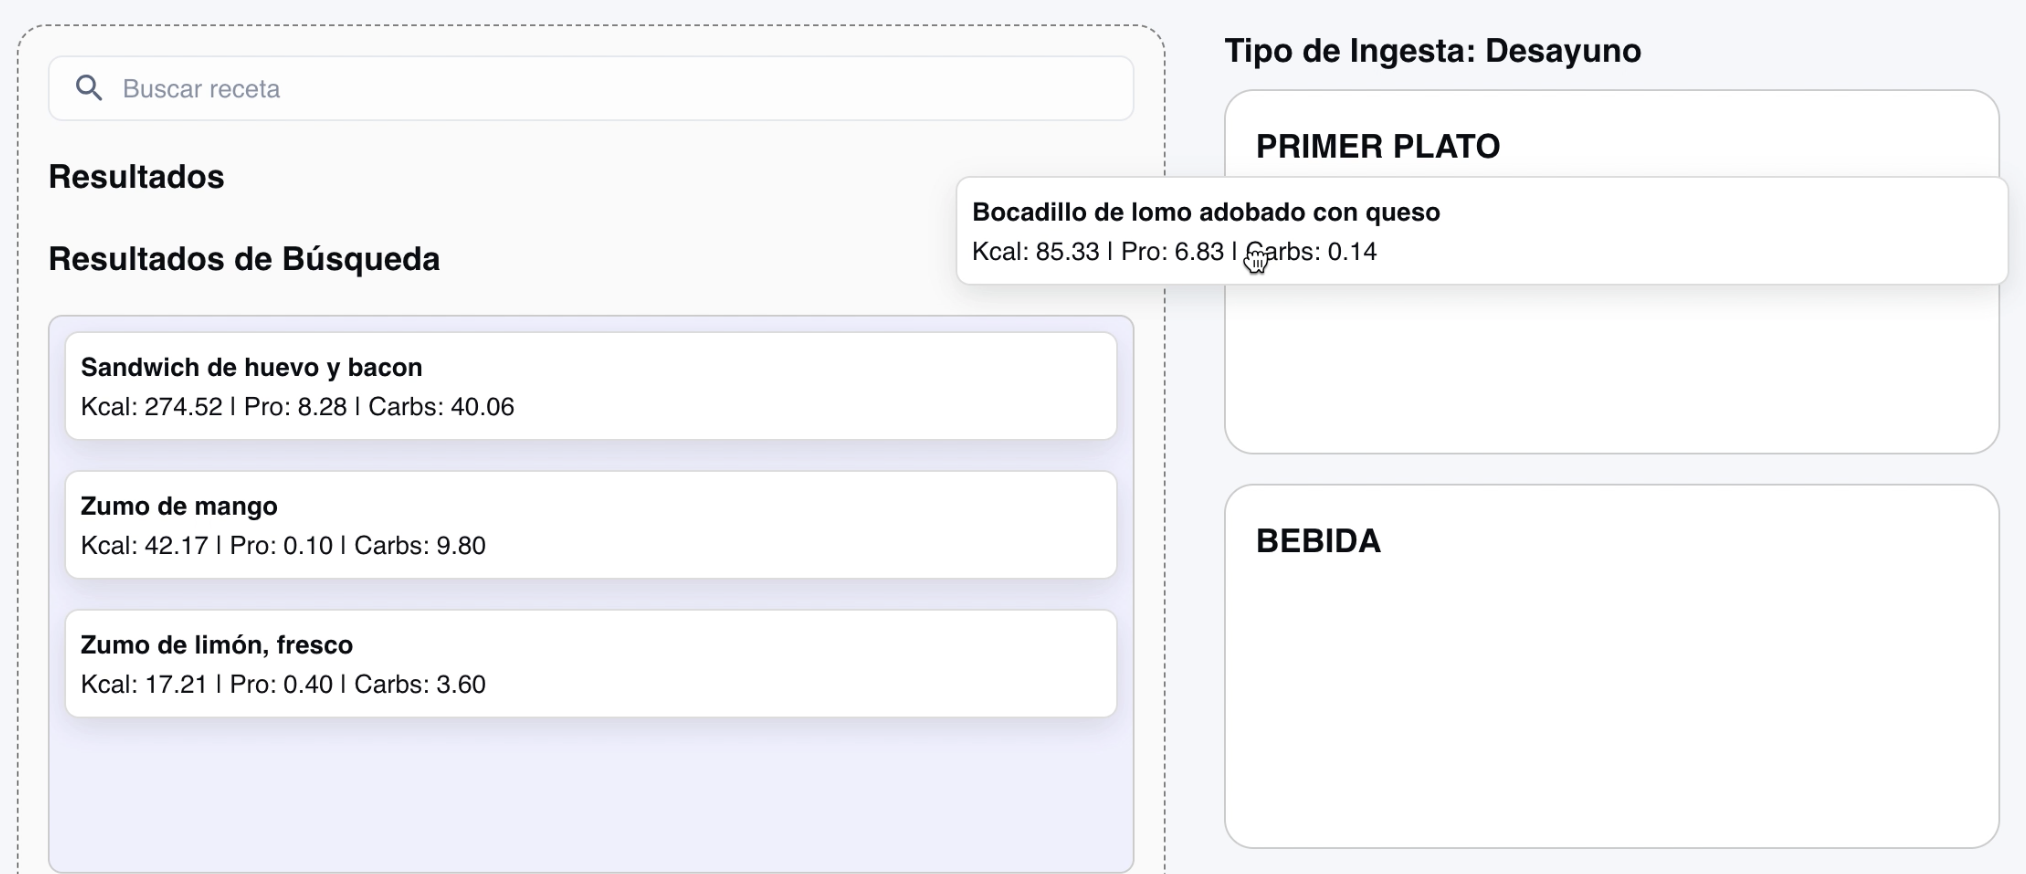
\includegraphics[width=1\linewidth]{Plantilla_TFG_latex//imagenes/drag_Drop.png}
    \caption{Interfaz de usuario con funcionalidad de arrastrar y soltar para la planificación de ingestas.}
    \label{fig:enter-label}
\end{figure}

Para ello, se integró la librería ``@dnd-kit'', que proporciona componentes reutilizables para definir elementos arrastrables (``Draggable'') y zonas receptivas (``Droppable''). A nivel técnico, el estado de las recetas y su organización se gestiona de forma controlada en React mediante estructuras de objetos dinámicos, con claves que combinan el tipo de ingesta y el tipo de receta (por ejemplo, ``almuerzo::postre''), lo que permite mantener múltiples niveles de agrupación y asegurar la coherencia en todo momento.

En el componente ``CrearIngestaForm.js'', el usuario puede buscar recetas a través de un campo de búsqueda unificado, que muestra sugerencias conectadas en tiempo real con el backend. Una vez seleccionada una receta, esta puede ser arrastrada hacia una de las cinco zonas de plato disponibles: entrante, primer plato, segundo plato, postre y bebida. Cada zona es visualmente distinta y mantiene su propia lista de recetas, que pueden reordenarse, eliminarse o reemplazarse fácilmente.

Por su parte, en el componente ``CrearDietaForm.js'' se extiende este mismo modelo a nivel semanal. Una vez seleccionados los días de la dieta y sus tipos de ingesta (por ejemplo, desayuno, almuerzo, cena), el usuario puede arrastrar ingestas completas hacia los días correspondientes. Esta lógica mantiene también el estado agrupado y estructurado por día y por tipo de ingesta, permitiendo planificar toda la semana de forma clara y organizada. Las ingestas ya existentes pueden reutilizarse gracias a un buscador similar, lo que agiliza la creación de planes dietéticos basados en patrones previos.

En ambos formularios, se incluyó compatibilidad con modo edición: al abrir una ingesta o dieta ya existente, el sistema reconstruye visualmente todas las zonas de arrastre y las recetas o ingestas asignadas, manteniendo la integridad de la planificación y permitiendo ajustes puntuales sin perder la estructura general.

Esta estrategia de implementación basada en ``drag-and-drop'' mejora significativamente la usabilidad, reduce los errores de entrada de datos y ofrece una experiencia centrada en la lógica visual.

\section{Otras herramientas utilizadas}

Además de los lenguajes de programación, bibliotecas y frameworks técnicos directamente empleados en el desarrollo del sistema, se han utilizado recursos complementarios que han contribuido de forma significativa a la redacción, planificación y desarrollo del Trabajo Fin de Grado.

\subsection*{Asistentes basados en inteligencia artificial}

Durante la elaboración de la memoria, se emplearon herramientas basadas en modelos de lenguaje para apoyar tareas de redacción técnica, generación de fragmentos de código y revisión estructural:

\begin{itemize}
    \item \textbf{ChatGPT (OpenAI)}~\cite{chatgpt}: Herramienta de asistencia basada en modelos de lenguaje desarrollados por OpenAI. 
    
    \item \textbf{DeepSeek}~\cite{deepseek}: Plataforma de modelos de lenguaje de código abierto especializada en generación de código, redacción técnica y razonamiento estructurado. 
\end{itemize}

\subsection*{Guía académica de referencia}

Asimismo, se ha seguido como referencia fundamental el documento elaborado por varios profesores de la Universidad de Granada, titulado \textit{Cómo escribir la memoria de tu TFG del Grado en Ingeniería Informática y presentarlo sin morir en el intento}~\cite{guillen2025memoria}. Esta guía ha sido clave para estructurar adecuadamente la memoria, definir los apartados requeridos y comprender las expectativas formales del Trabajo Fin de Grado según los criterios académicos establecidos. Además, ha servido de orientación a lo largo de todo el proceso, desde la planificación inicial hasta la fase final de redacción y revisión, y ha resultado especialmente útil para preparar la defensa oral del proyecto, al ofrecer recomendaciones prácticas sobre la exposición pública, el uso de recursos visuales y la organización del discurso.

\subsection*{Reutilización de código y estructuras}

En el desarrollo de este sistema también se reutilizó parte del código fuente del proyecto \texttt{foodDB}~\cite{fooddb}, adaptando parte de su estructura de base de datos documental. A pesar de esta reutilización inicial, se realizaron modificaciones sustanciales para ajustarse a los requisitos funcionales y de dominio del presente sistema.

Además, en la fase inicial del desarrollo del frontend, se empleó como base parte del código proporcionado por las plantillas oficiales de \texttt{Material UI}~\cite{mui_templates}, en particular aquellas orientadas a sistemas de autenticación y paneles administrativos. Estas plantillas ofrecidas gratuitamente por el equipo de MUI sirvieron como punto de partida para construir la interfaz, que luego fue personalizada según las necesidades del sistema.

\section{Conclusión}
En resumen, este capítulo ha presentado de forma detallada el proceso de implementación del sistema propuesto, abordando tanto los aspectos técnicos como las decisiones prácticas adoptadas durante el desarrollo. Se ha explicado cómo la arquitectura basada en React, FastAPI y MongoDB ha permitido construir una solución modular, escalable y mantenible, capaz de integrar todas las funcionalidades planteadas. Todo el código fuente desarrollado en este proyecto, incluyendo tanto el backend, el frontend y los scripts de configuración, se encuentra disponible en el repositorio público del Trabajo Fin de Grado: 
\url{https://github.com/ugritai/nutridiet}.
